\documentclass{beamer}

% Theme and Color Scheme
\usetheme{Boadilla}
\usecolortheme{seahorse}
\setbeamersize{text margin left=0.5cm, text margin right=0.5cm}
\setbeamertemplate{footline}{}
\date{}

% Required Packages
\usepackage{graphicx}
\usepackage{amsmath, amssymb}
\usepackage{booktabs}
\usepackage[authoryear,round]{natbib} % author–year citations
\usepackage{qrcode}
\usepackage{listings}
\lstset{
  basicstyle=\ttfamily\scriptsize,
  breaklines=true,
  showstringspaces=false,
  columns=fullflexible,
  upquote=true
}
\usepackage{tikz}
\usetikzlibrary{positioning,arrows.meta,fit,calc,shadows.blur}

% ===== Presenter notes toggle (Overleaf-friendly) =====
\usepackage{pgfpages}
\newif\ifpresenter
\presentertrue    % <— uncomment for PRESENTER PDF (two-panel pages)
% \presenterfalse     % <— audience PDF (slides only)

\ifpresenter
  \setbeameroption{show notes on second screen=right}
  \setbeamerfont{note page}{size=\small}
  \setbeamercolor{note page}{bg=black!3}
\else
  \setbeameroption{hide notes}
\fi
% ======================================================

% Title Page Information
\title[RMSTSS]{RMSTSS: A Comprehensive Software Suite for Power and Sample Size Calculation in Modern Clinical Trials}
\author{Arnab Aich}
\institute{Florida State University}
\date{\today}

\begin{document}

% ---------- Frame 1: Title Page ----------
\begin{frame}
  \titlepage
  \note{
  \textbf{Opening (10s).} Hi everyone, thanks for being here. I’m Arnab Aich from Florida State University. Today I’ll walk you through \textbf{RMSTSS}, a practical toolkit for planning survival trials when proportional hazards may not hold. \\
  \textbf{Agenda (10s).} We’ll start with motivation, then the RMST idea and causal interpretation, followed by models, power/sample size methods, two examples, and a quick tour of the web app. \\
  \textbf{Transition (2s).} Let’s begin with the \emph{why}.
  }
\end{frame}

% ---------- Frame 2 ----------
\begin{frame}
\frametitle{The Fundamental Goal: Planning Better Clinical Trials}

\begin{block}{Two Questions Every Trial Must Answer}
\begin{enumerate}
  \item How many participants are needed? \textbf{(sample size)}
  \item What is the chance of detecting a true effect?\textbf{(power)}
\end{enumerate}
\end{block}

\vspace{0.6em}

\begin{block}{Why This Matters}
\begin{itemize}
  \item \textbf{Ethics:} Avoid underpowered or unnecessary studies.
  \item \textbf{Efficiency:} Trials are costly—careful design saves time and resources.
  \item \textbf{Science:} Adequate power is essential for trustworthy conclusions.
\end{itemize}
\end{block}

\note{
\textbf{Set-up (20s).} Trial planning always starts with two decisions: sample size and power. These are not just technicalities—underpowered studies can waste participant effort and money, and overpowered studies can be unnecessarily large. \\
\textbf{Pause (2s).} Emphasize ethical and scientific responsibility. \\
\textbf{Transition (2s).} With that context, let’s review the standard survival setup.
}
\end{frame}

% ---------- Frame 3 ----------
\begin{frame}
\frametitle{The Standard Approach: Survival Models}
In many trials, the outcome is the \textbf{time until an event} occurs (e.g., recovery, disease progression, death).

\begin{block}{Key Notations}
\begin{itemize}
    \item $T$: The true time-to-event for a subject.
    \item $C$: The censoring time (e.g., end of study, patient drops out).
    \item We observe $Y = \min(T, C)$ and an event indicator $\delta$.
    \item \textbf{Survival Function}, $S(t) = P(T > t)$: The probability of surviving past time $t$.
    \item \textbf{Hazard Function}, $h(t)$: The instantaneous risk of the event at time $t$, given survival up to $t$.
    $$h(t) = \lim_{\Delta t \to 0} \frac{P(t \le T < t + \Delta t \mid T \ge t)}{\Delta t} = \frac{f(t)}{S(t)}$$
\end{itemize}
\end{block}

\note{
\textbf{Scaffolding (20s).} We observe $Y=\min(T,C)$ with indicator $\delta$. Survival $S(t)$ and hazard $h(t)$ summarize event-time behavior. \\
\textbf{Pause (1s).} This is standard—but it sets us up for a common problem with the next slide. \\
\textbf{Transition (1s).} Let’s talk hazards and proportionality.
}
\end{frame}

% ---------- Frame 4 ----------
\begin{frame}
\frametitle{Proportional Hazards (PH) and Hazard Ratio Issues}

\begin{columns}[T,onlytextwidth]
  %%% Left column: Assumption + image %%%
  \begin{column}{0.48\textwidth}
    \begin{block}{PH Assumption}
      Treatment hazard is a constant multiple of control:
      \[
        h_1(t) = h_0(t)\cdot \theta
      \]
    \end{block}

    \centering
    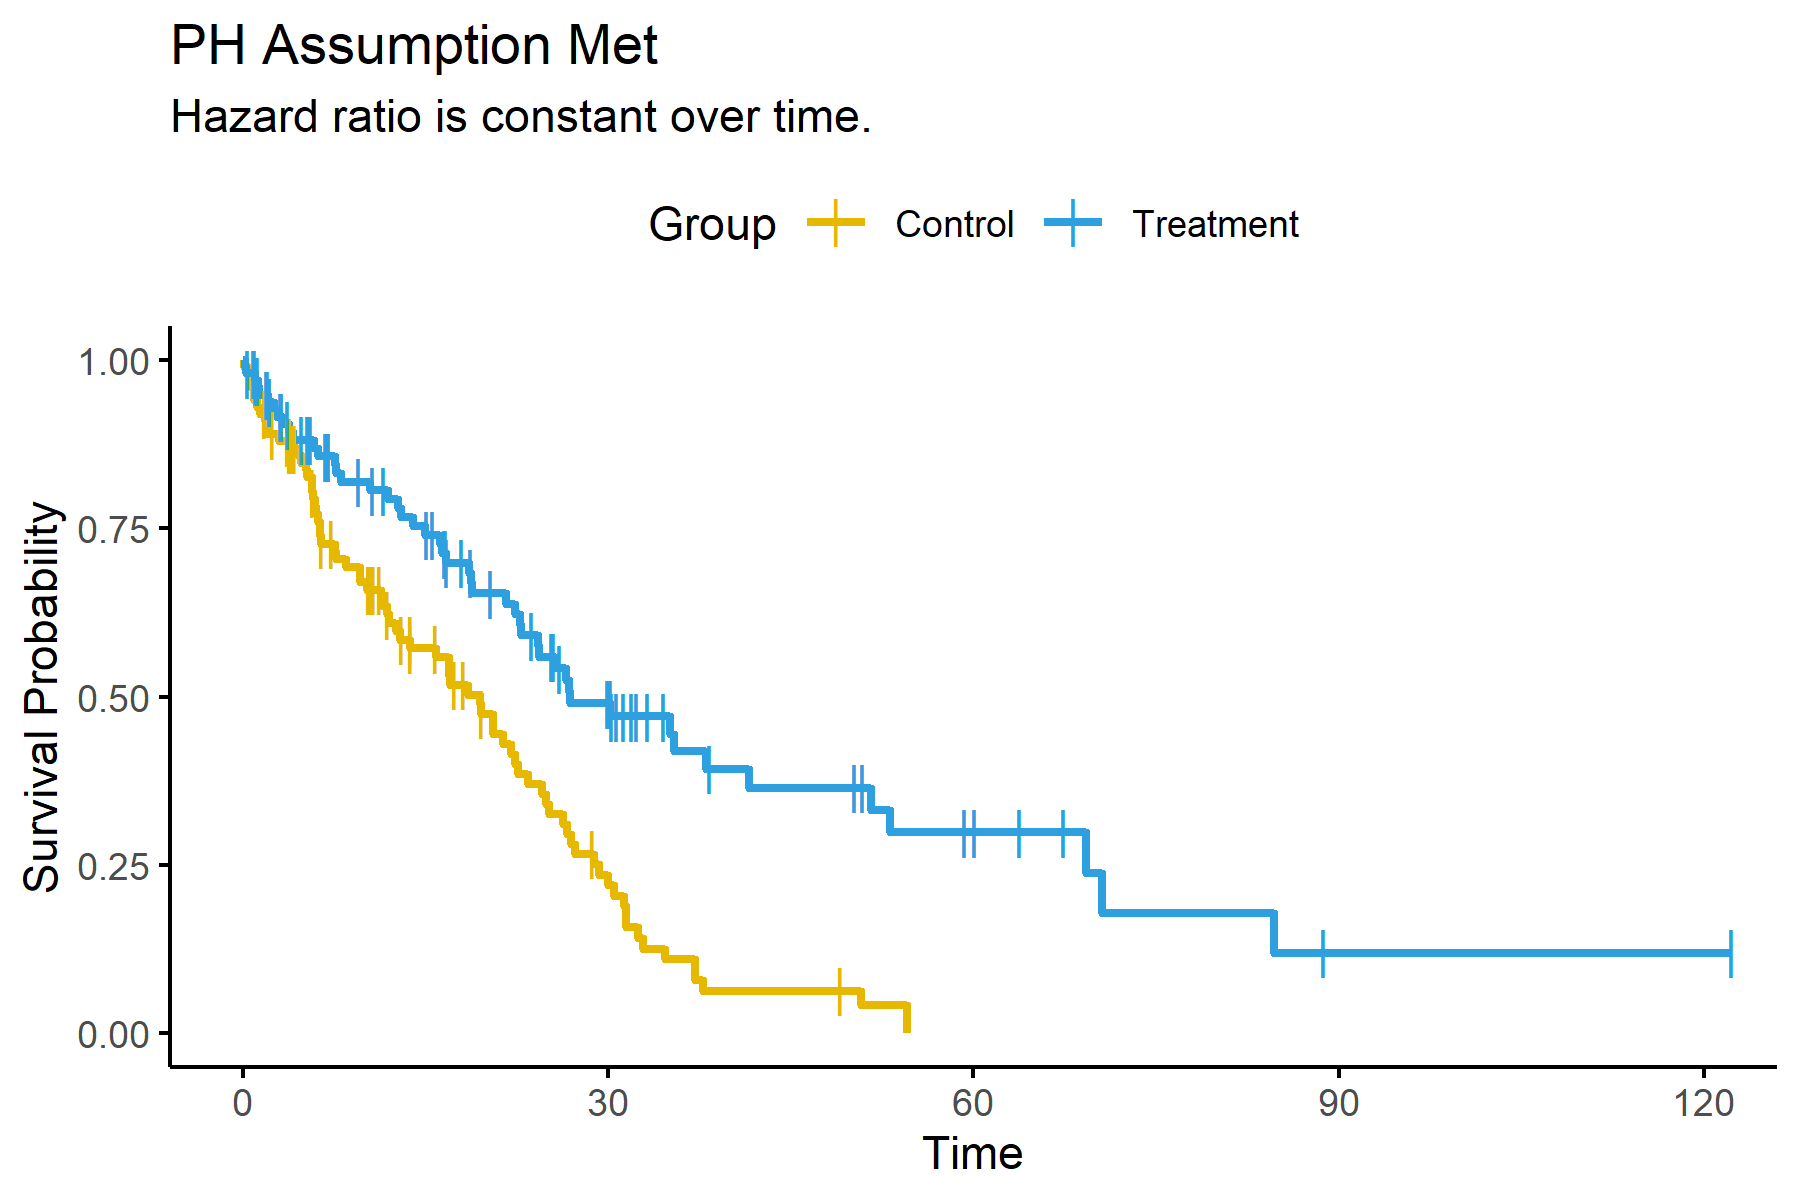
\includegraphics[width=\linewidth,height = 0.9\linewidth]{images/ph_assumption_met.png} 
  \end{column}

  \hspace{0.04\textwidth}

  %%% Right column: Problems + image %%%
  \begin{column}{0.48\textwidth}
    \begin{block}{Problems with HR}
      \begin{itemize}
        \item PH often fails (delayed effects, waning benefit, crossing curves).
        \item No Causal interpretation.
      \end{itemize}
    \end{block}
    \centering
    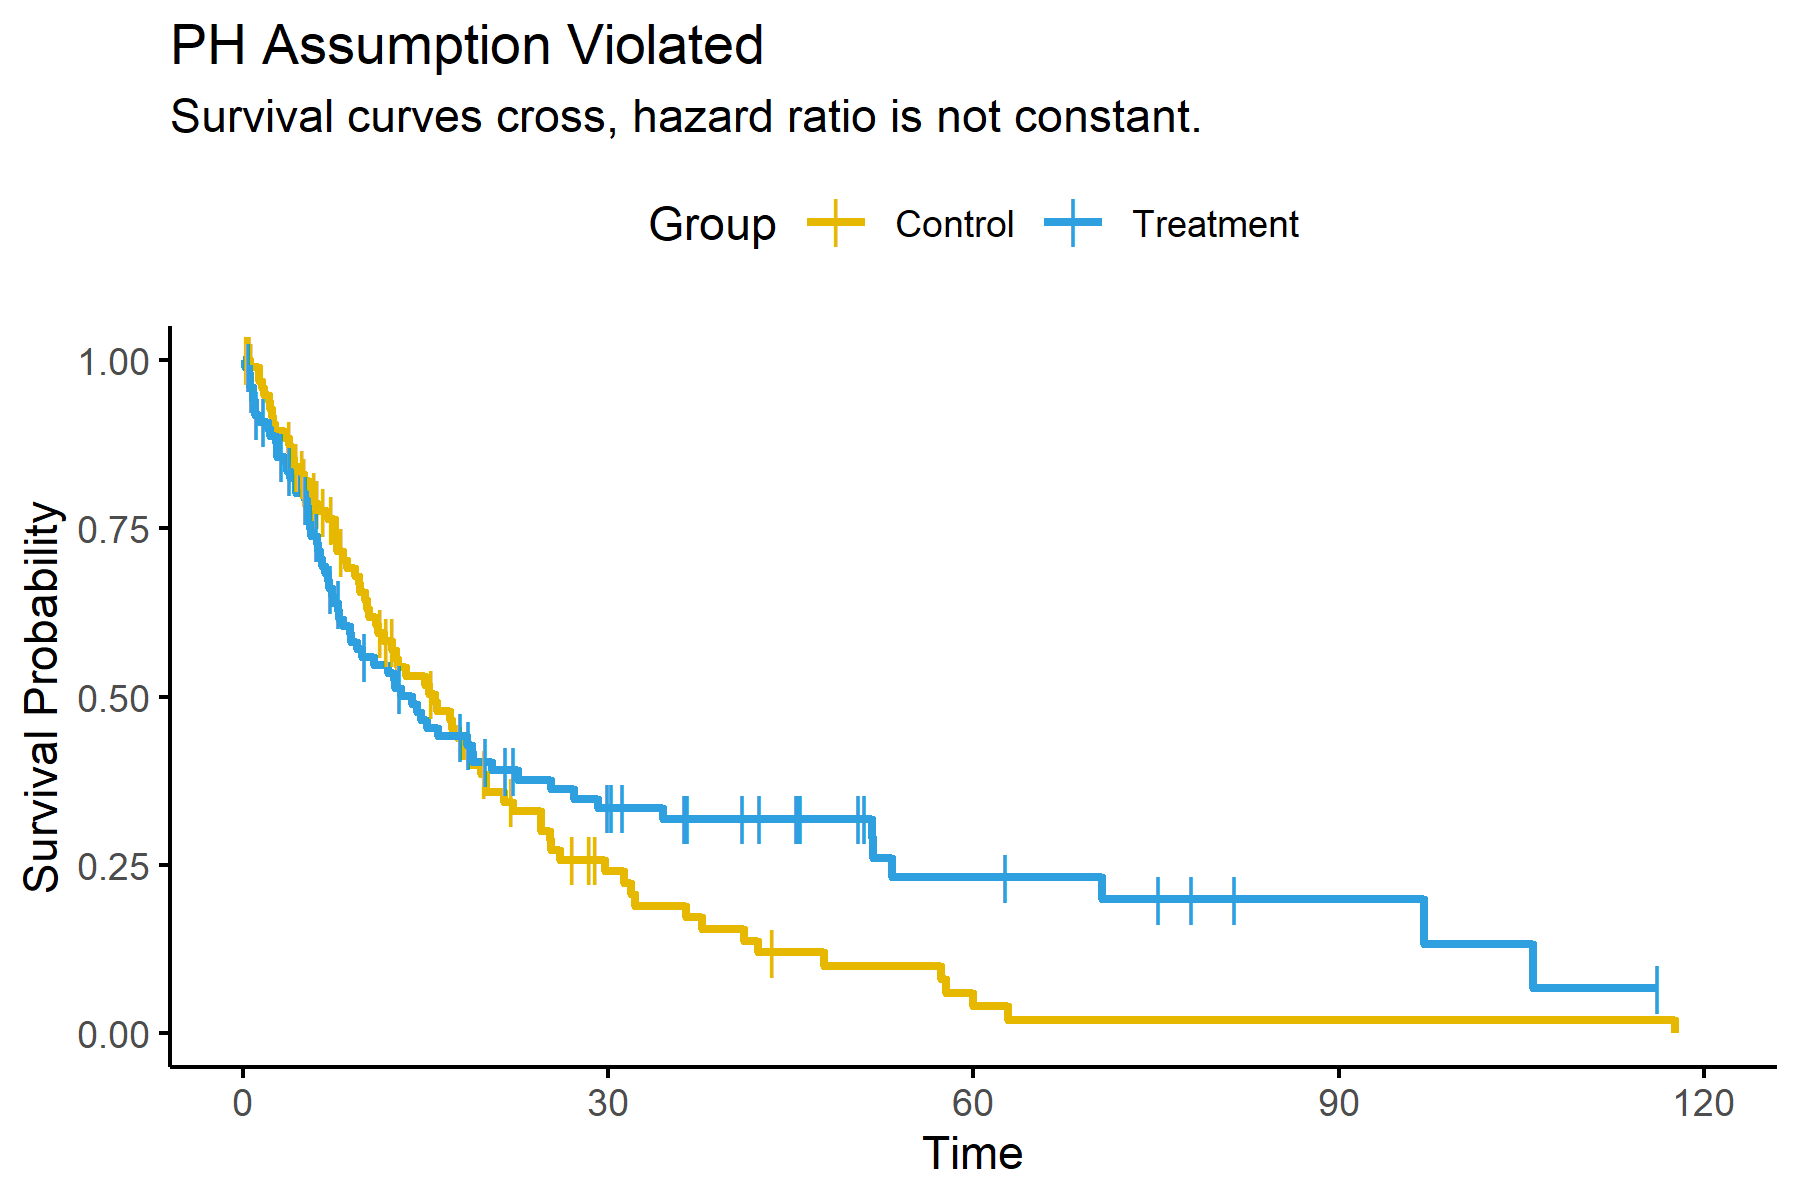
\includegraphics[width=\linewidth,height = 0.9\linewidth]{images/ph_assumption_violated.png} 
  \end{column}
\end{columns}

\note{
\textbf{Key point (25s).} PH says hazards differ by a constant factor. It’s elegant, but in modern trials we often see delayed treatment effects, diminishing effects, or crossing curves—so the hazard ratio becomes a time-averaged number with murky interpretation. \\
\textbf{Pause (2s).} We need something interpretable when PH fails. \\
\textbf{Transition (1s).} That’s where RMST helps.
}
\end{frame}

% ---------- Frame 5 ----------
\begin{frame}
\frametitle{The Solution: Restricted Mean Survival Time (RMST)}
\begin{block}{Definition}
The RMST is the average event-free survival time up to a pre-specified time point, $L$. It is the area under the survival curve from 0 to $L$.
$$\mu(L) = E[\min(T, L)] = \int_0^L S(t) dt$$
\end{block}

\begin{block}{Interpretation \& Advantages}
\begin{itemize}
    \item \textbf{Directly Interpretable:} It provides a clear, absolute measure of survival in units of time.
    \item \textbf{No Proportional Hazards Assumption:} The RMST is a non-parametric measure, making it a valid and robust choice even when survival curves cross.
    \item \textbf{Clinically Meaningful:} It quantifies the average time gained or lost, which is highly relevant to both clinicians and patients.
\end{itemize}
\end{block}

\note{
\textbf{Essence (20s).} RMST tells us “how much event-free time, on average, up to time $L$.” It’s robust to non-proportional hazards and communicates in time units—intuitive for clinicians and patients. \\
\textbf{Transition (2s).} Next, the causal estimand we target.
}
\end{frame}

% ---------- Frame 6 ----------
\begin{frame}
\frametitle{Causal Interpretation of RMST Difference}
\begin{block}{}
\[
\Delta(L) = \mu_{\text{treat}}(L) - \mu_{\text{control}}(L)
\]

\begin{itemize}
  \item $\Delta(L)$ quantifies the \textbf{average gain in event-free time} from treatment over $[0,L]$.  
  \item Interpreted directly in \textbf{time units} (e.g., “3 extra months without progression”).  
  \item The treatment effect is the \textbf{difference in area under the survival curves} up to $L$.  
\end{itemize}
\end{block}

% Bottom row: two images, no titles/captions
\begin{columns}[T,onlytextwidth]
  \begin{column}{0.5\textwidth}
    \centering
    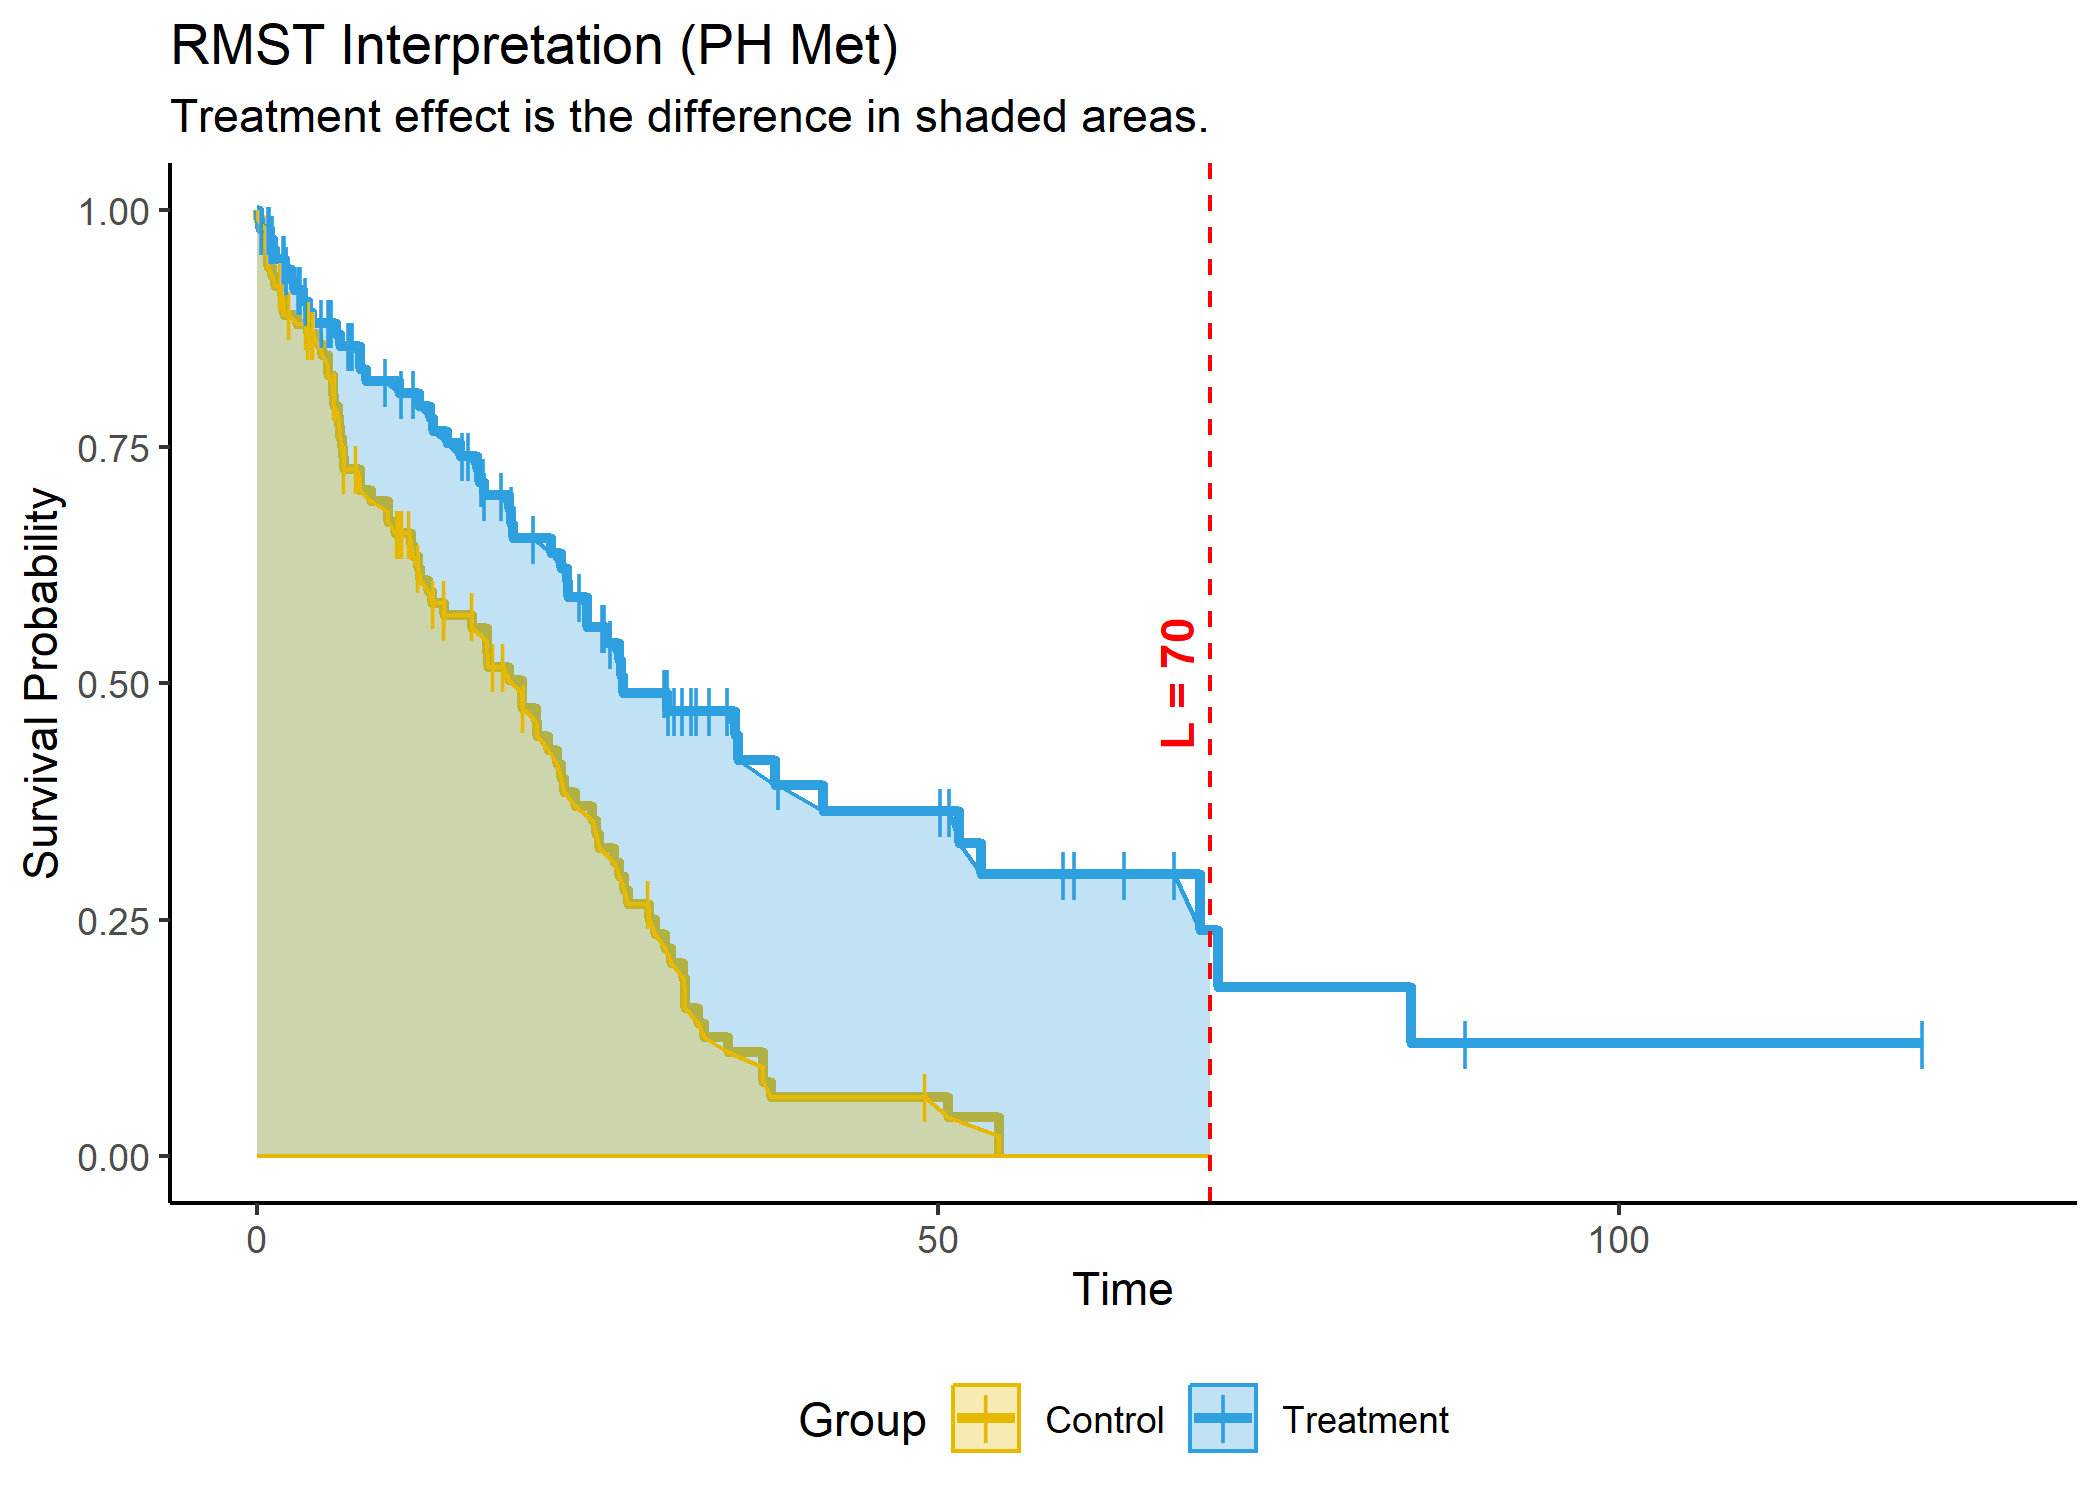
\includegraphics[width=\textwidth, height=0.7\textwidth]{images/rmst_causal_plot_ph_met.png}
  \end{column}
  \begin{column}{0.5\textwidth}
    \centering
    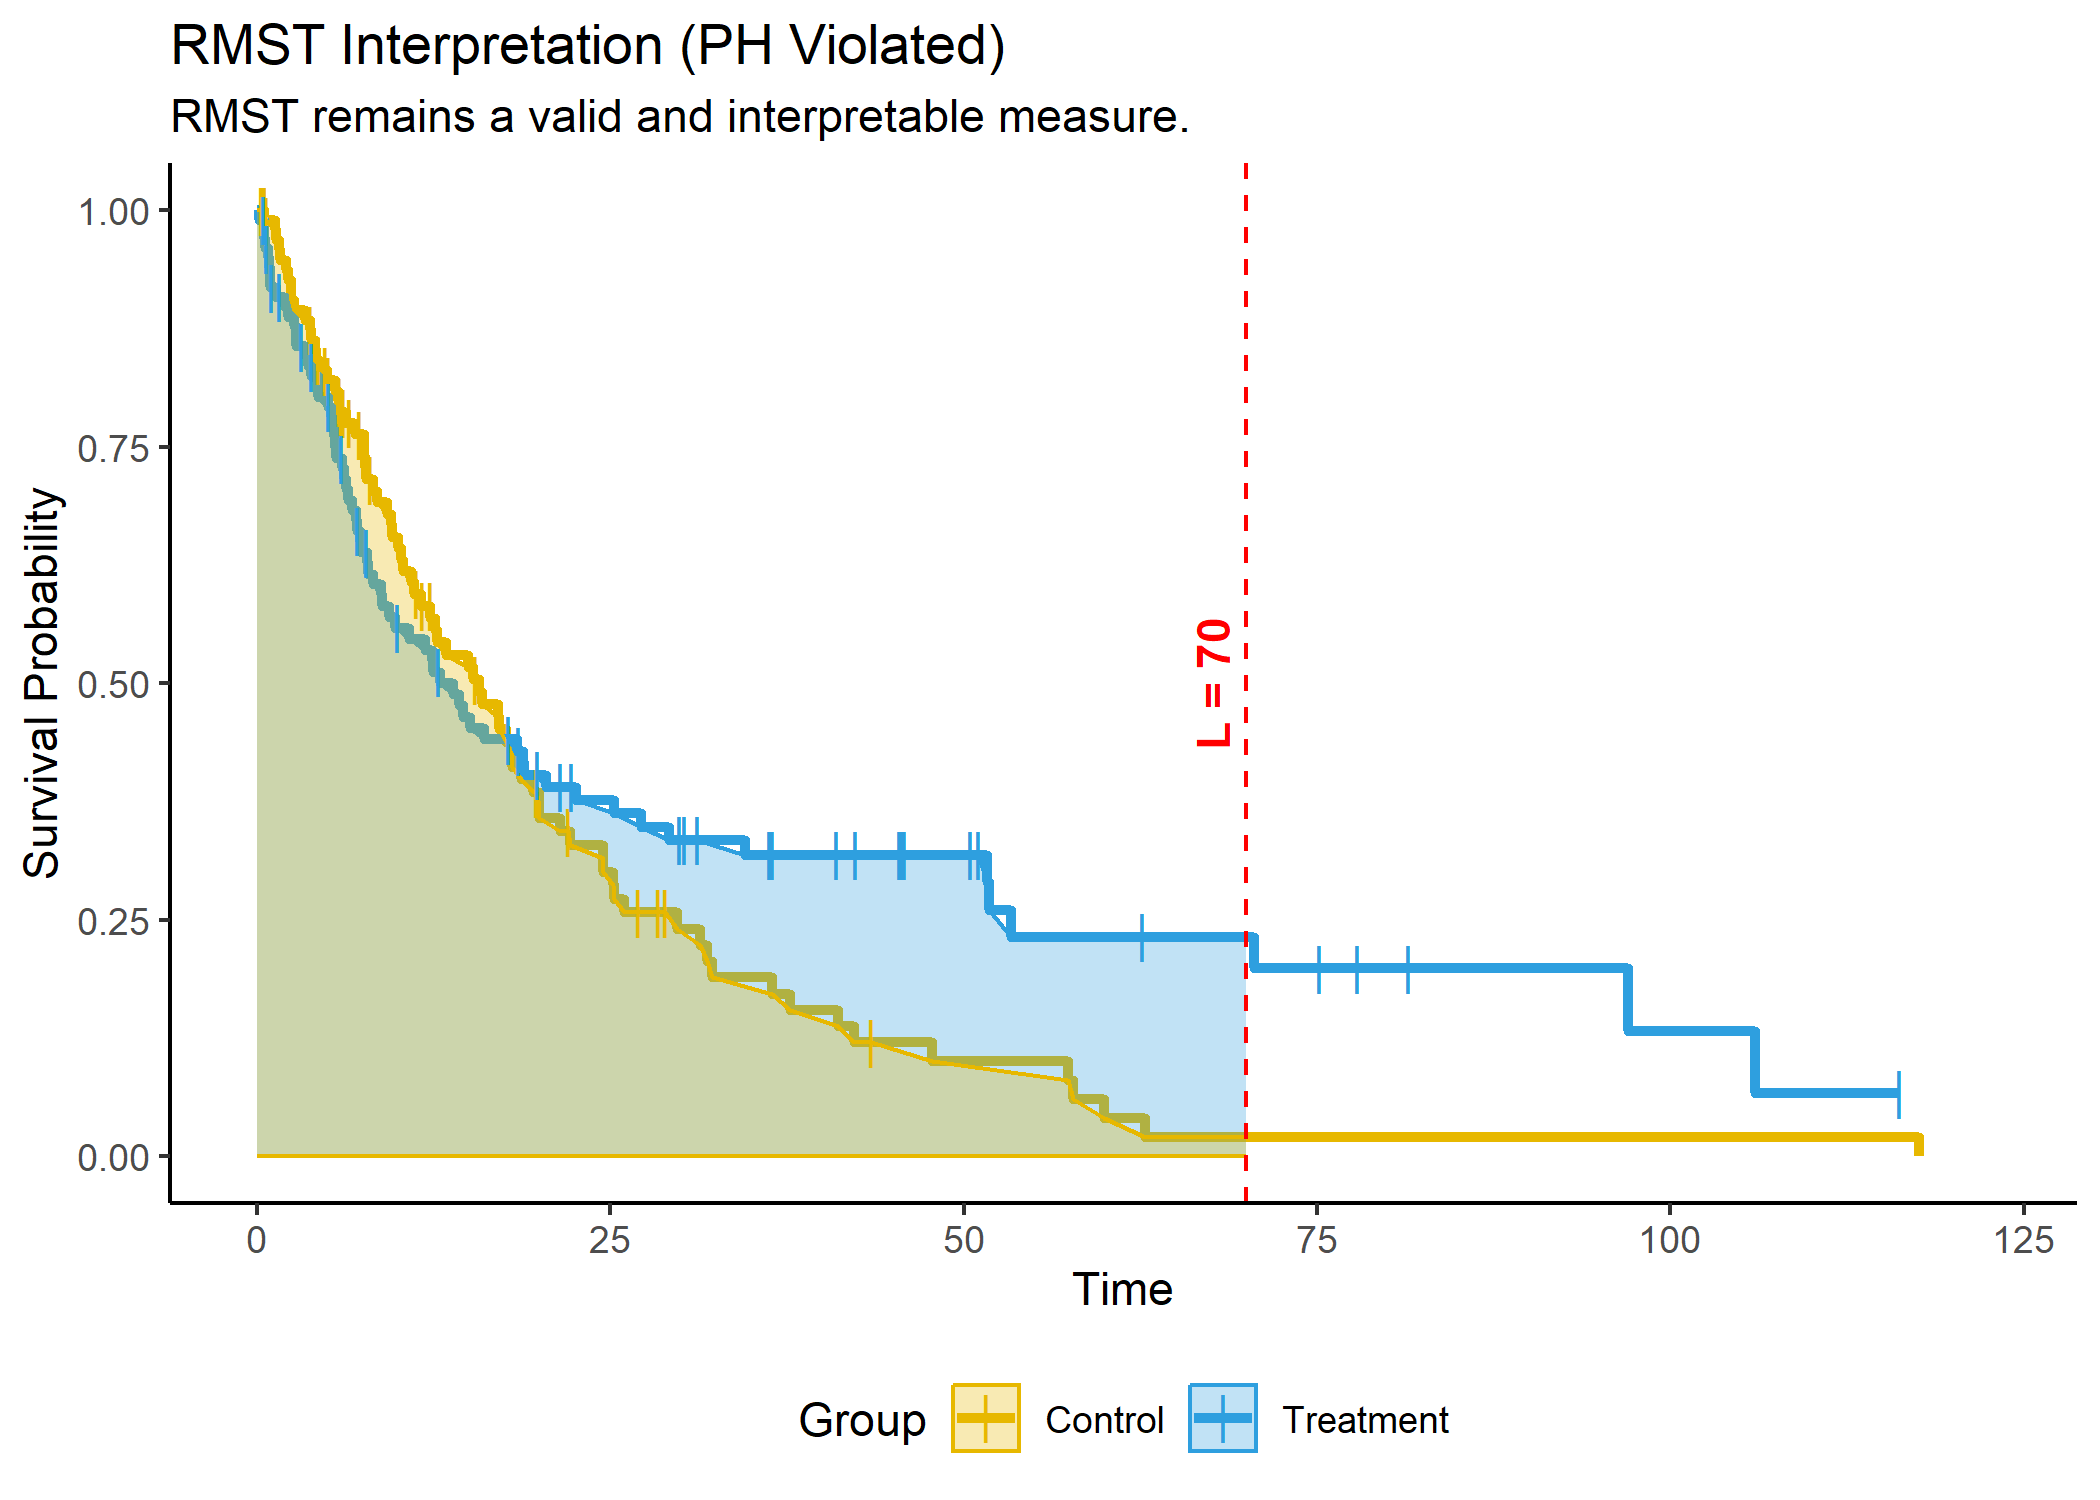
\includegraphics[width=\textwidth, height=0.7\textwidth]{images/rmst_causal_plot_ph_violated.png}
  \end{column}
\end{columns}

\note{
\textbf{Takeaway (20s).} Our treatment effect is the RMST difference: the average extra event-free time up to $L$. Visually, it’s the difference in the \emph{areas} under the survival curves. This remains valid whether PH holds or not. \\
\textbf{Pause (2s).} With the estimand set, let’s talk models and software.
}
\end{frame}

% ---------- Frame 7 ----------
\begin{frame}
\frametitle{Bridging Gap: Theory and Implementation}

\begin{block}{We Provide:}
\scriptsize
\begin{itemize}
  \item Unified framework for \textbf{RMST-based power and sample size} calculations.
  \item \textbf{RMSTSS R package}: open-source, reproducible implementation.
  \item \textbf{RMSTSS Shiny web app}: user-friendly interface, no coding required.
\end{itemize}
\end{block}
\textit{The following models are currently available.}
\begin{figure}
    \centering
    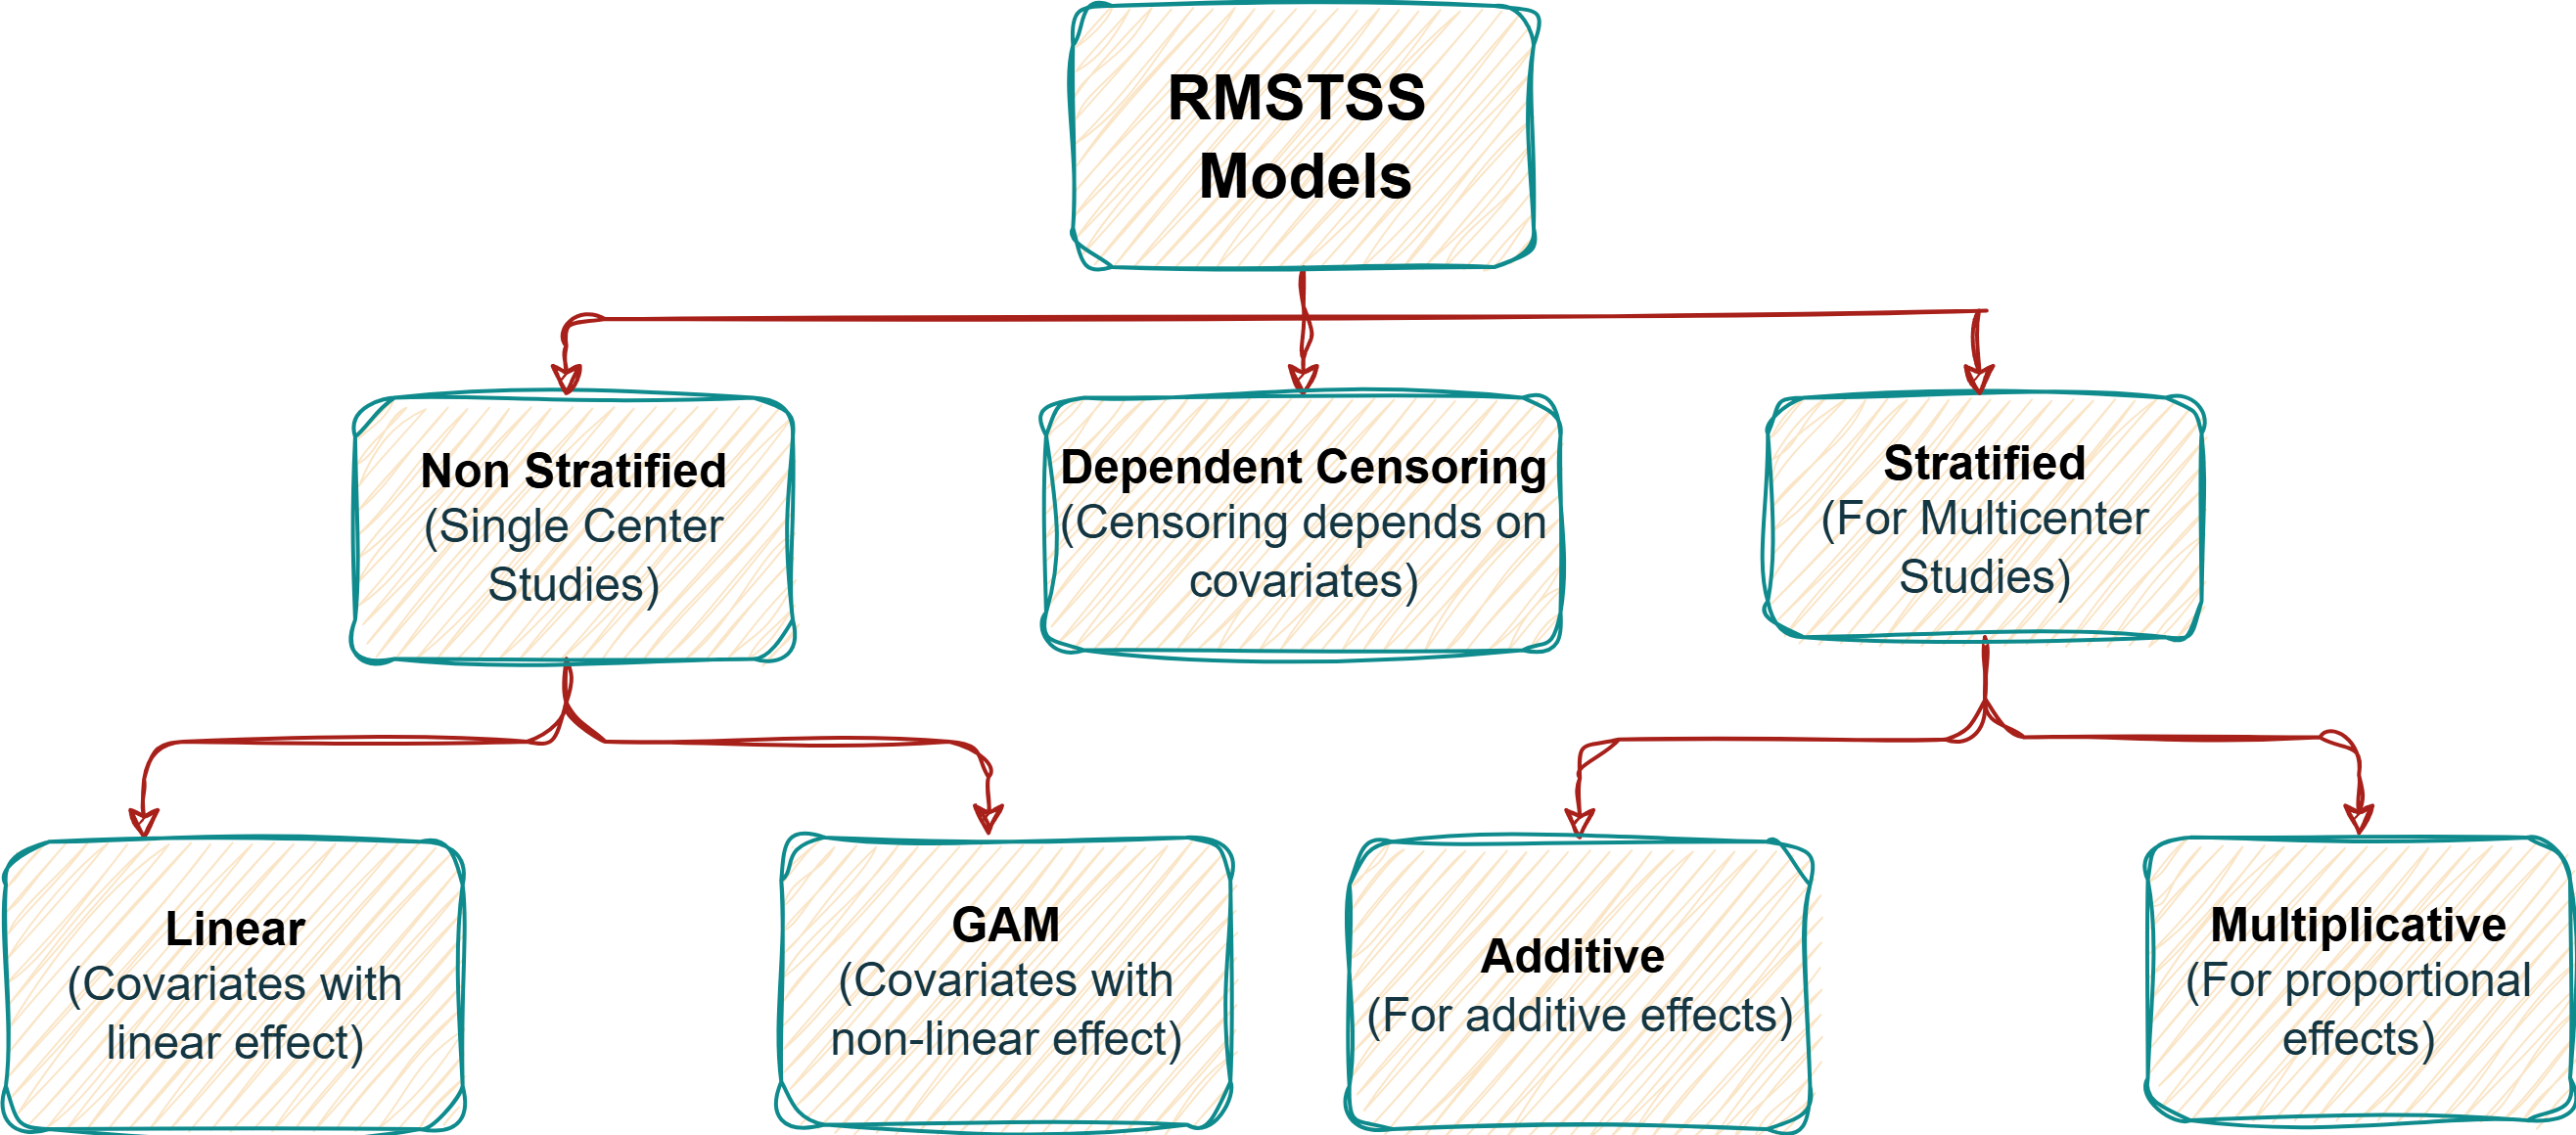
\includegraphics[width=1\linewidth]{images/app-models.png}
\end{figure}

\note{
\textbf{Bridge (15s).} We packaged RMST-based design in an R package and a Shiny web app. The goal: make robust, interpretable planning accessible. \\
\textbf{Cue (2s).} Now the modeling pieces.
}
\end{frame}

% ---------- Frame 8 ----------
\begin{frame}
\frametitle{Notation and Linear RMST Model}

\begin{block}{Observed Data}
For subject $i=1,\dots,n$:  
\begin{itemize}
  \item $Y_i = \min(T_i, C_i)$: observed follow-up time  
  \item $\delta_i = \mathbb{1}(T_i \le C_i)$: event indicator  
  \item $A_i \in \{0,1\}$: treatment group  
  \item $Z_i$: baseline covariates
\end{itemize}
\end{block}

\begin{block}{Linear RMST Model}
\[
E[\min(T_i,L) \mid A_i, Z_i] = \beta_0 + \beta_A A_i + \beta_Z^\top Z_i
\]

\begin{itemize}
  \item $\beta_A$: adjusted RMST difference between treatment arms  
  \item Direct regression not feasible due to censoring $\Rightarrow$ need IPCW
\end{itemize}
\end{block}

\note{
\textbf{Model (20s).} A simple linear mean model targets the RMST difference. Because of censoring, we cannot regress naively on observed $Y_i$; we use IPCW or pseudo-observations. \\
\textbf{Transition (2s).} First, IPCW.
}
\end{frame}

% ---------- Frame 9 ----------
\begin{frame}
\frametitle{Simple Linear IPCW Model \citep{zhao2001}}

\begin{block}{Censoring Distribution}
Let $G(t) = P(C_i > t)$ be the survival function of censoring time.  
We estimate $\widehat{G}(t)$ using Kaplan–Meier.
\end{block}

\begin{block}{Weights}
Each subject receives weight
\[
w_i = \frac{\delta_i}{\widehat{G}(Y_i)}.
\]
\end{block}

\begin{block}{Weighted Least Squares}
Estimate $\beta$ by minimizing
\[
\widehat{\beta} = \arg\min_\beta \sum_{i=1}^n w_i \Big\{ Y_i - (\beta_0 + \beta_A A_i + \beta_Z^\top Z_i)\Big\}^2.
\]
\end{block}

\note{
\textbf{IPCW (20s).} IPCW re-weights uncensored observations by the inverse censoring probability so the weighted sample mimics full follow-up. Under standard assumptions, the regression recovers unbiased estimates of $\beta_A$. \\
\textbf{Pause (2s).} Alternate route: pseudo-observations with GAM.
}
\end{frame}

% ---------- Frame 10 ----------
\begin{frame}
\frametitle{Generalized Additive Model \citep{parner2010}}

\begin{block}{Pseudo-Observations}
\[
\text{pseudo}_i(L) = n \cdot \widehat{\mu}(L) - (n-1)\cdot \widehat{\mu}^{(-i)}(L),
\]
\scriptsize
where $\widehat{\mu}(L)$ is the RMST estimate from the full sample and  
$\widehat{\mu}^{(-i)}(L)$ is the estimate with subject $i$ removed.  

\textbf{Key Property:}  
\[
E[\text{pseudo}_i(L)] = E[\min(T_i,L)]
\]
$\Rightarrow$ pseudo-observations can be treated as uncensored outcomes.
\end{block}

\begin{block}{Semiparametric GAM Model}
\[
E[\text{pseudo}_i(L)] = \beta_0 + \beta_A A_i + \sum_{k=1}^q f_k(Z_{ik}),
\]
\scriptsize
where $f_k(\cdot)$ are spline-based smooth functions.

\begin{itemize}
  \item $\beta_A$: adjusted RMST difference between treatment arms.  
  \item Handles censoring via pseudo-observations.  
  \item Captures nonlinear covariate effects flexibly while preserving interpretability.  
\end{itemize}
\end{block}
\note{
\textbf{GAM route (20s).} Pseudo-observations yield “uncensored-like” outcomes, so we can use a GAM for flexibility. We retain $\beta_A$ as the RMST difference while letting covariate effects be nonlinear. \\
\textbf{Transition (2s).} Next, stratified models.
}
\end{frame}

% ---------- Frame 11 ----------
\begin{frame}
\frametitle{Stratified Models \citep{royston2011}}

\begin{block}{Additive Model}
Assume each stratum $j$ has its own baseline $\alpha_j$, with a common treatment effect:
\[
E[\min(T_i,L) \mid A_i, S_i=j] = \alpha_j + \beta_A A_i + \beta_Z^\top Z_i.
\]
Interpretation: $\beta_A$ is the constant added survival time across strata.
\end{block}

\begin{block}{Multiplicative Model}
Assume proportional treatment effect across strata:
\[
E[\min(T_i,L) \mid A_i, S_i=j] = \mu_{0j}(L) \cdot \exp(\beta_A A_i + \beta_Z^\top Z_i).
\]
Interpretation: $\exp(\beta_A)$ is the RMST ratio (treatment vs. control), common across strata.
\end{block}

\note{
\textbf{Choice (15s).} Additive model answers “how many months gained?”; multiplicative answers “what ratio of RMST?”. Pick what clinicians find most natural. \\
\textbf{Transition (2s).} Censoring may also depend on covariates—handle that next.
}
\end{frame}

% ---------- Frame 12 ----------
\begin{frame}
\frametitle{Dependent Censoring}

\frametitle{Dependent Censoring \citep{robins2000}}

\begin{block}{Problem}
If censoring depends on covariates, a single $\widehat{G}(t)$ is biased.
\end{block}

\begin{block}{Solution: Cause-Specific Models}
For $K$ censoring causes, fit cause-specific hazards $\lambda_{Ck}(t \mid Z)$ and cumulative hazards $\Lambda_{Ck}(t \mid Z)$.  
Then
\[
\widehat{G}(t \mid Z) = \exp\!\Big(-\sum_{k=1}^K \widehat{\Lambda}_{Ck}(t \mid Z)\Big).
\]
\end{block}

\begin{block}{IPCW with Dependent Censoring}
Use $\widehat{G}(t \mid Z)$ in the IPCW weights.
\end{block}

\note{
\textbf{Point (15s).} When censoring relates to covariates or causes, model that structure so the weights are valid. This protects against bias from informative dropout. \\
\textbf{Transition (2s).} Now, how we do power and sample size.
}
\end{frame}

% ---------- Frame 13 ----------
\begin{frame}
\frametitle{Power and Sample Size Calculation}


\begin{block}{Analytical Approach}
Uses asymptotic variance of the estimated treatment effect:
\[
\text{Power} = 
\Phi\!\left( 
\frac{|\widehat{\beta}_A|}{\widehat{\sigma}_{\beta_A}/\sqrt{n}} - z_{1-\alpha/2}
\right),
\]
where $\widehat{\sigma}_{\beta_A}$ is the estimated standard error and $\Phi$ is the standard normal CDF.
\end{block}

\begin{block}{Bootstrap Approach}
Simulation-based resampling from pilot data:
\[
\text{Power} =
\frac{\#\{\text{replicates with $p$-value} < \alpha\}}{B},
\]
where $B$ = number of bootstrap replicates.
\end{block}

\note{
\textbf{Contrast (20s).} Analytical is fast and great for scanning sample sizes; bootstrap is flexible and validates power under complex settings. In RMSTSS we support both, often using analytical to search and bootstrap to confirm. \\
\textbf{Transition (2s).} Let’s see two examples.
}
\end{frame}

% ---------- Frame 14 ----------
\begin{frame}[fragile]{Example 1: Linear IPCW RMST Model}
\textbf{Goal:} Analytic sample size search for RMST difference under a linear IPCW model.

\begin{columns}[T,onlytextwidth]
  \begin{column}{0.55\textwidth}
  \scriptsize
\begin{lstlisting}[language=R]
ss_results_vet <- linear.ss.analytical(
  pilot_data     = vet,
  time_var       = "time",
  status_var     = "status",
  arm_var        = "arm",
  target_power   = 0.40,
  linear_terms   = "karno",
  L              = 365,
  n_start        = 1000,
  n_step         = 250,
  max_n_per_arm  = 5000
)
\end{lstlisting}
{\scriptsize
\textbf{Parameter Notes:} \\
\texttt{n\_start} – starting sample size per arm. \\
\texttt{n\_step} – increment at each step. \\
\texttt{max\_n\_per\_arm} – upper cap considered. \\
}
  \end{column}
  \begin{column}{0.45\textwidth}
    \centering
    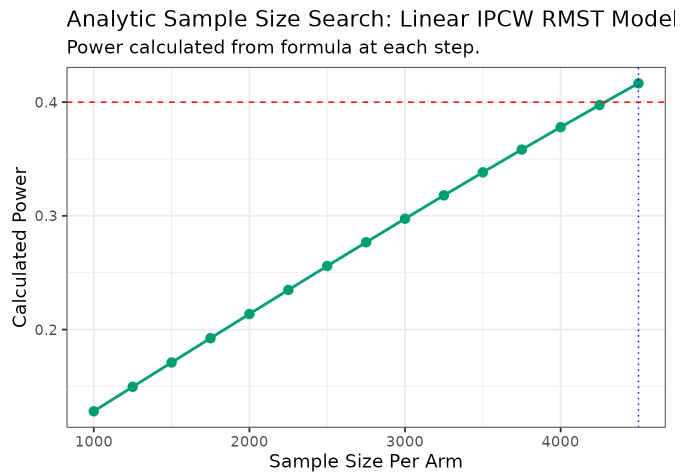
\includegraphics[width=\linewidth]{images/Example_LIN.png}

    \vspace{0.4em}
    \footnotesize
   \textbf{Simulation Summary}

    \vspace{0.25em}
 \begin{tabular}{@{}ll@{}}
      \toprule
      \texttt{Statistic} & \texttt{Value} \\
      \midrule
       RMST Difference  & -3.966558 \\
      \bottomrule
    \end{tabular}
  \end{column}
\end{columns}

\note{
\textbf{Story (25s).} Using the veteran dataset, we target 40\% power at $L=365$ adjusting for Karnofsky score. We scan from 1000 per arm in steps of 250 up to 5000. Power increases steadily; around 4500 per arm we reach the target. Focus on workflow and reproducibility rather than the specific number. \\
\textbf{Pause (2s).} Now a stratified bootstrap example.
}
\end{frame}

% ---------- Frame 15 ----------
\begin{frame}[fragile]{Example 2: Multiplicative Stratified RMST Model}
\textbf{Goal:} Estimate power for treatment effect on RMST ratio across strata using bootstrap.

\begin{columns}[T,onlytextwidth]
  \begin{column}{0.6\textwidth}
  \scriptsize
\begin{lstlisting}[language=R]
power_ms_boot <- MS.power.boot(
  pilot_data     = colon_death,
  time_var       = "time",
  status_var     = "status",
  arm_var        = "arm",
  strata_var     = "strata",
  sample_sizes   = c(100, 300, 500),
  L              = 1825,
  n_sim = 100, n_start = 100, n_step = 50,
  patience = 4, parallel.cores = 10
)
\end{lstlisting}
{\scriptsize
\textbf{Parameter Notes:} \\
\texttt{n\_sim}: \# bootstrap replicates. \\
\texttt{n\_start}: initial size/stratum; \texttt{n\_step}: increment. \\
\texttt{patience}: iterations allowed without improvement. \\
\texttt{parallel.cores}: cores for parallelism. \\
}
  \end{column}
  \begin{column}{0.4\textwidth}
    \centering
    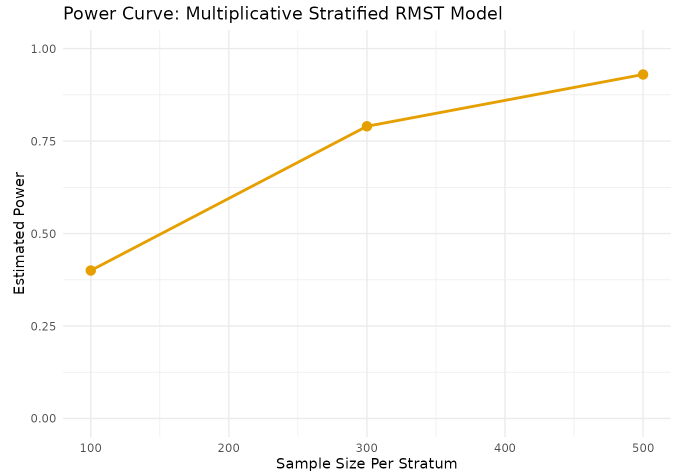
\includegraphics[width=\linewidth]{images/Example_MS.png}

    \vspace{0.4em}
    \footnotesize
    \textbf{Simulation Summary}

    \vspace{0.25em}
    \begin{tabular}{@{}ll@{}}
      \toprule
      Statistic        & Value \\
      \midrule
      Mean RMST Ratio  & 1.0065 \\
      95\% CI Lower    & 0.9680 \\
      95\% CI Upper    & 1.0572 \\
      \bottomrule
    \end{tabular}
  \end{column}
\end{columns}

\note{
\textbf{Narrative (25s).} With stratification, we bootstrap power for the RMST ratio over a horizon of five years ($L=1825$). The mean ratio is about 1.0065, CI roughly 0.968–1.057 in this pilot. This demonstrates the workflow; real planning would refine assumptions and sample sizes. \\
\textbf{Transition (2s).} Now the web app.
}
\end{frame}

% ---------- Frame 16 ----------
\begin{frame}
\frametitle{Application Interface}
\begin{figure}
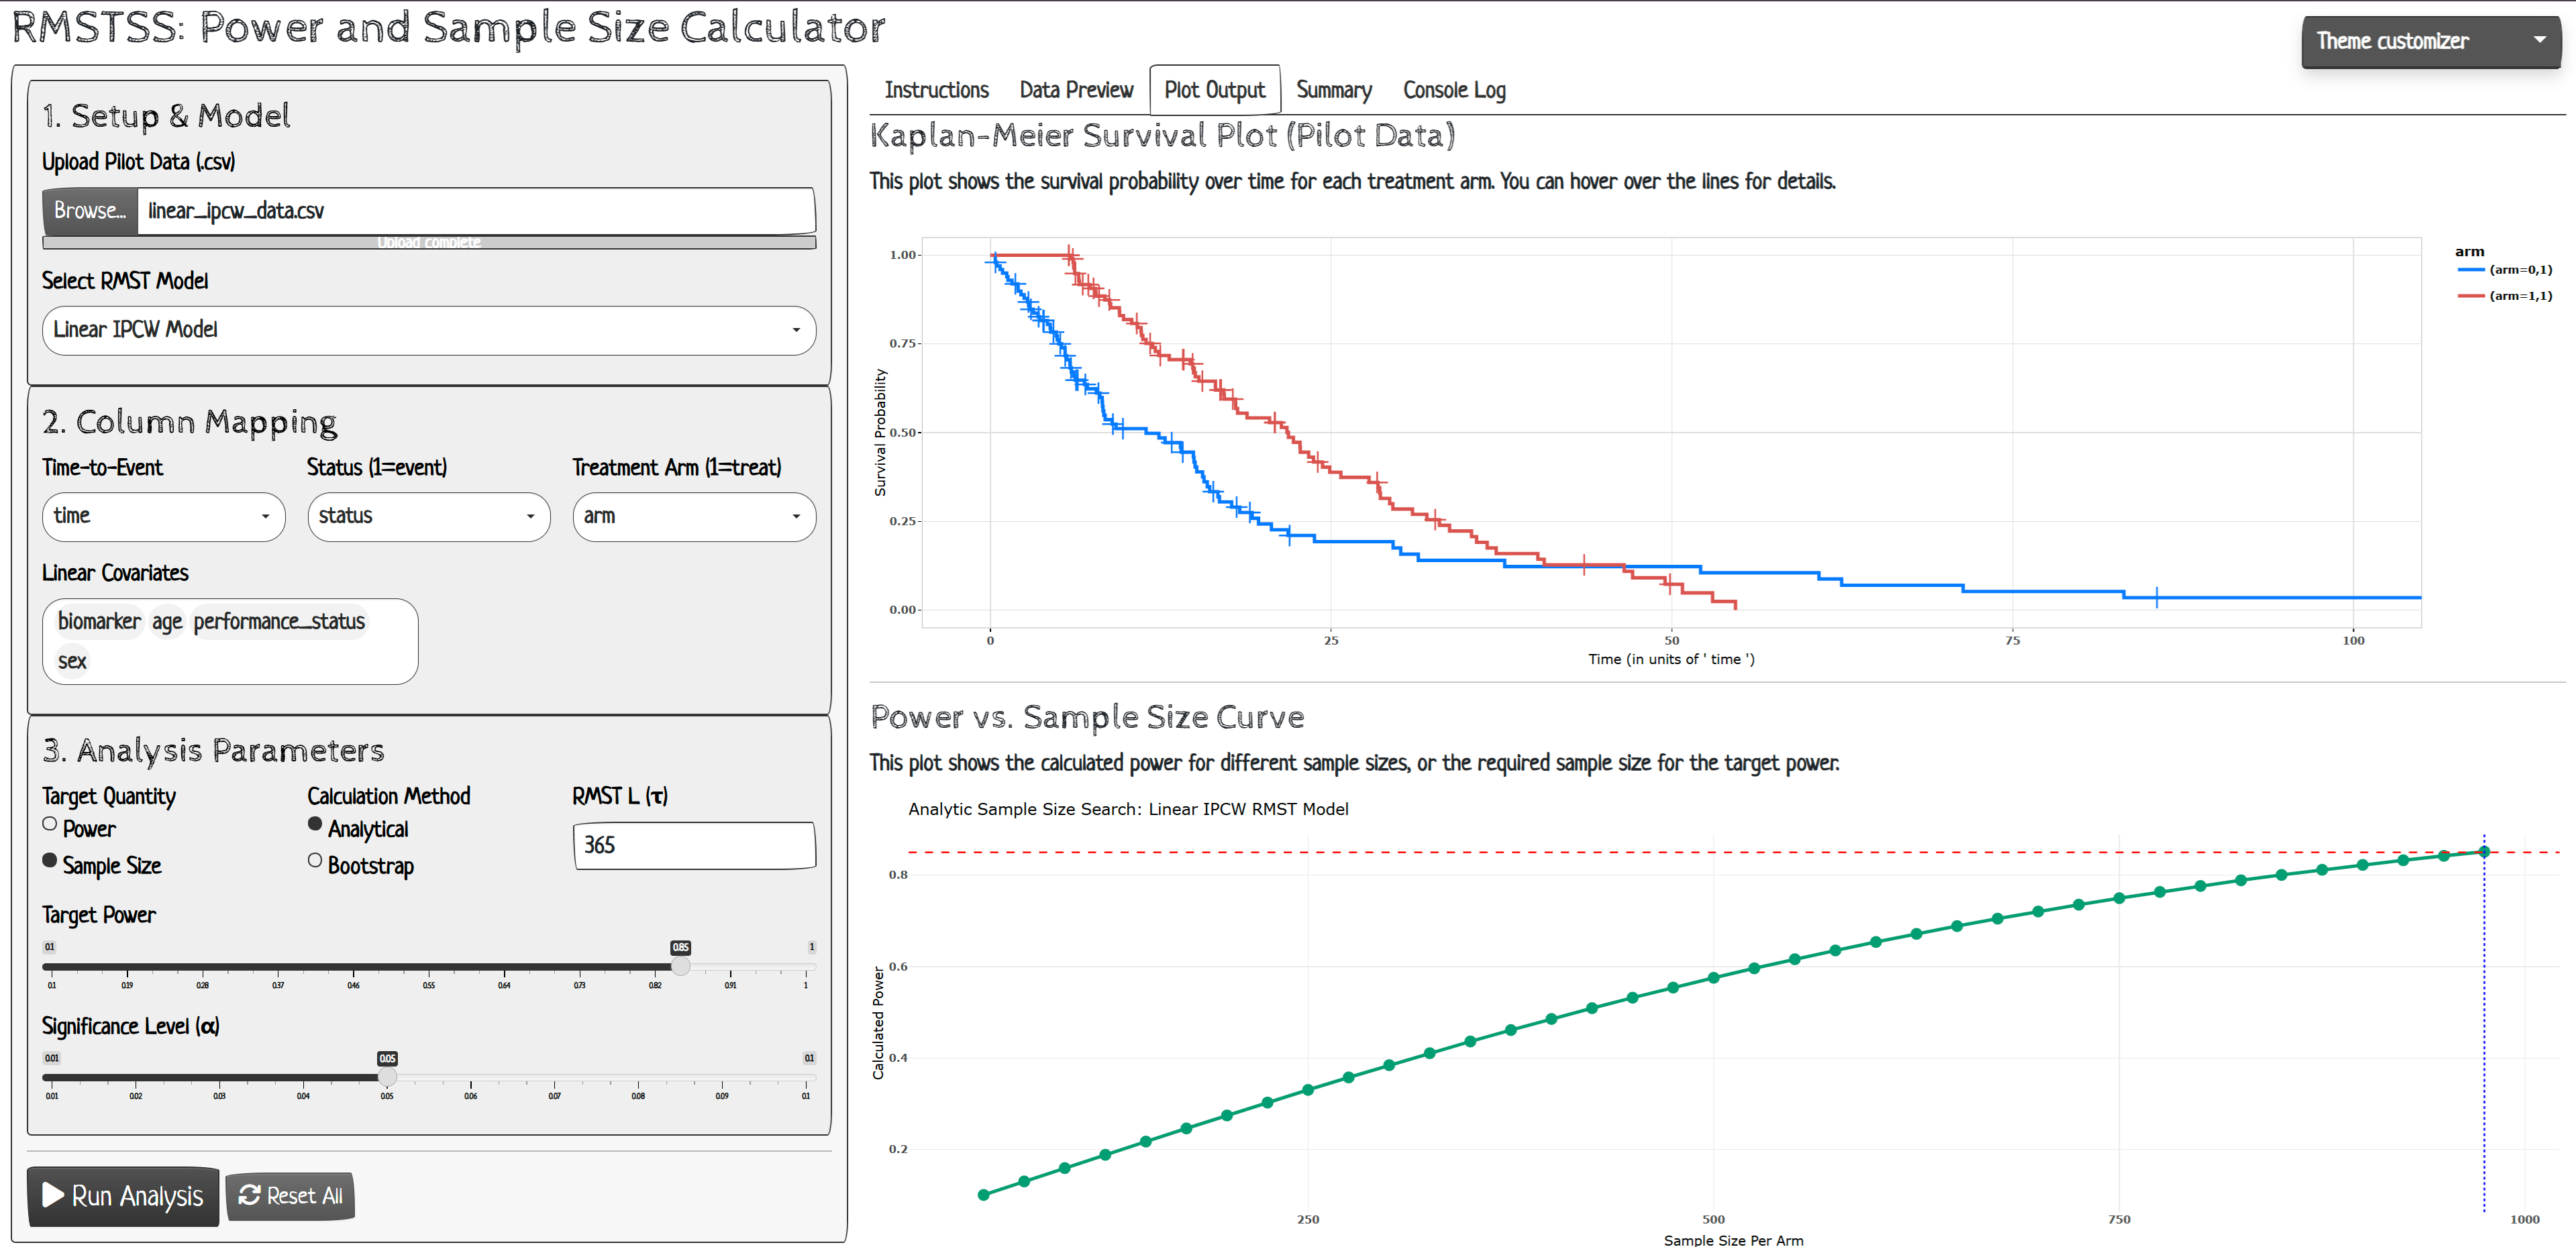
\includegraphics[width=\textwidth, height = 0.65\textwidth]{images/app-ss.png}
\end{figure}

\note{
\textbf{Tour (15s).} The Shiny app lets you upload CSVs, map columns, pick models/goals/methods, and view interactive outputs. This reduces friction for collaborators who prefer a GUI over R code. \\
\textbf{Transition (2s).} Quick feature recap.
}
\end{frame}

% ---------- Frame 17 ----------
\begin{frame}
\frametitle{RMSTSS: Web Application Feature}

\centering
\scalebox{0.8}{%
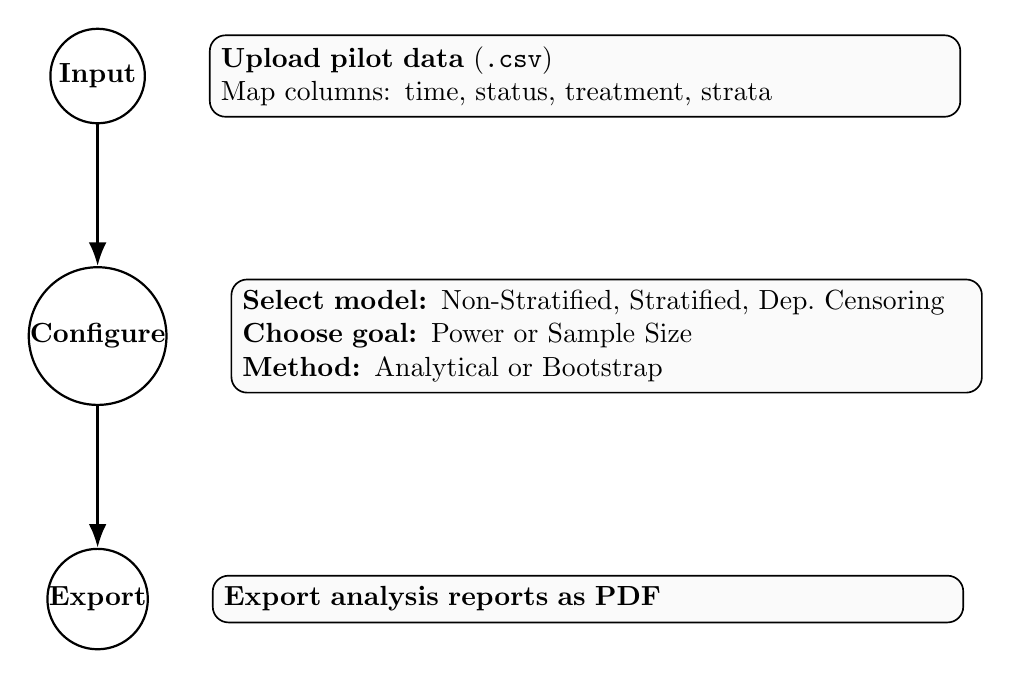
\begin{tikzpicture}[
  node distance=10mm and 8mm,
  bubble/.style={
    circle, draw, line width=0.8pt,
    minimum size=12mm, inner sep=0pt, font=\bfseries
  },
  box/.style={
    rectangle, rounded corners=2mm, draw, line width=0.6pt,
    align=left, inner sep=4pt, text width=9.25cm, fill=black!2
  },
  arr/.style={-{Latex[length=3mm]}, line width=1.pt}
]

% Row 1
\node[bubble] (b1) {Input};
\node[box, right=8mm of b1] (bx1) {%
  \textbf{Upload pilot data} (\texttt{.csv})\\
  Map columns: time, status, treatment, strata
};

% Row 2
\node[bubble, below=18mm of b1] (b2) {Configure};
\node[box, right=8mm of b2] (bx2) {%
  \textbf{Select model:} Non-Stratified, Stratified, Dep.\ Censoring\\
  \textbf{Choose goal:} Power or Sample Size \\
  \textbf{Method:} Analytical or Bootstrap
};

% Row 3
\node[bubble, below=18mm of b2] (b3) {Export};
\node[box, right=8mm of b3] (bx3) {%
  \textbf{Export analysis reports as PDF}
};

\draw[arr] (b1.south) -- (b2.north);
\draw[arr] (b2.south) -- (b3.north);
\end{tikzpicture}%
}

\begin{itemize}
\centering
    \item \textbf{Fully web-based} — no R installation required
    \item \textbf{Interactive} plots and \textbf{customizable} visual themes
\end{itemize}

\note{
\textbf{Summary (15s).} The workflow is simple: Input → Configure → Export. You can visualize survival/power curves and customize styling. It’s fully web-based—no local R setup required. \\
\textbf{Transition (2s).} Final thoughts.
}
\end{frame}

% ---------- Frame 18 ----------
\begin{frame}
\frametitle{Conclusion \& Future Aims}

\begin{block}{Conclusion}
\begin{itemize}
  \item \textbf{Statistically Rigorous:} linear, GAM, dependent censoring, stratified RMST
  \item \textbf{Causally Interpretable:} $\beta_A$ (difference) or $\exp(\beta_A)$ (ratio)
  \item \textbf{Practical:} R package + Shiny app
\end{itemize}
\end{block}

\begin{block}{Future Aims}
\begin{itemize}
  \item Time-varying treatments and adaptive designs
  \item Pilot-free planning via data generation
  \item Multi-arm/platform trial modules
\end{itemize}
\end{block}

\note{
\textbf{Wrap (20s).} RMSTSS aims to make robust, interpretable planning routine. We support multiple models and both analytical and bootstrap power/SS calculations, in code and via a GUI. \\
\textbf{Pause (2s).} Next, access and credits.
}
\end{frame}

% ---------- Frame 19 ----------
\begin{frame}
\frametitle{Access \& Acknowledgments}
\begin{columns}[T]
\begin{column}{0.5\textwidth}
\scriptsize
    \textbf{Acknowledgments}
 \begin{itemize}
        \item Grateful appreciation to Dr.\ Yuan Zhang (UTHSC) for mentorship
        \item Special thanks to Dr.\ Gregory Farage and Dr.\ Saunak Sen (UTHSC) for guidance and support
        \item Support provided by UTHSC BERD
        \item Research funded by NSF Grant No.\ 2220726
    \end{itemize}
\vfill
\begin{center}
\Huge{\textbf{Questions?}}
\end{center}
\end{column}
\begin{column}{0.5\textwidth}
\scriptsize
\centering
\textbf{Scan for Web App} \\
\qrcode[height=3cm]{https://arnab96.shinyapps.io/uthsc-app/}
\vspace{2em}\\
\textbf{Scan for R Package} \\
\qrcode[height=3cm]{https://uthsc-zhang.github.io/RMSTSS-Package/}
\end{column}
\end{columns}

\note{
\textbf{Close (20s).} Thanks to our mentors and collaborators, and to the funding support acknowledged here. The QR codes link to the live web app and package documentation. I’m happy to take questions. \\
\textbf{Optional pause (3s).} Invite discussion on use cases or integration in ongoing trials.
}
\end{frame}

% ---------- References (optional slide) ----------
\begin{frame}
\frametitle{References}
\scriptsize
\bibliographystyle{plainnat}
\bibliography{references}
\note{
Use author–year citations. If you’d rather hide this slide for time, you can comment it out; the in-slide citations will still render names/years.
}
\end{frame}

\end{document}
